\documentclass[12pt]{article}
\usepackage[utf8]{inputenc}
\usepackage[spanish]{babel}
\usepackage{amsmath, amssymb, amsfonts}
\usepackage{graphicx}
\usepackage{booktabs}
\usepackage{geometry}
\usepackage{float}
\geometry{a4paper, margin=1in}
\title{Reporte de Identificación y Análisis del Péndulo Doble}
\author{Pipeline Automatizado}
\date{\today}

\begin{document}
\maketitle

\section{Descripción del Sistema}
El sistema analizado es un péndulo doble: dos masas \(m_1\) y \(m_2\) conectadas por barras rígidas de longitudes \(L_1\) y \(L_2\), que oscilan libremente bajo la acción de la gravedad. Posee dos grados de libertad: los ángulos \(\theta_1\) y \(\theta_2\). El modelo se obtiene aplicando las ecuaciones de Euler-Lagrange. Los parámetros se identifican a partir de un video usando tracking YOLO y optimización multi-shooting.

\begin{figure}[H]
\centering
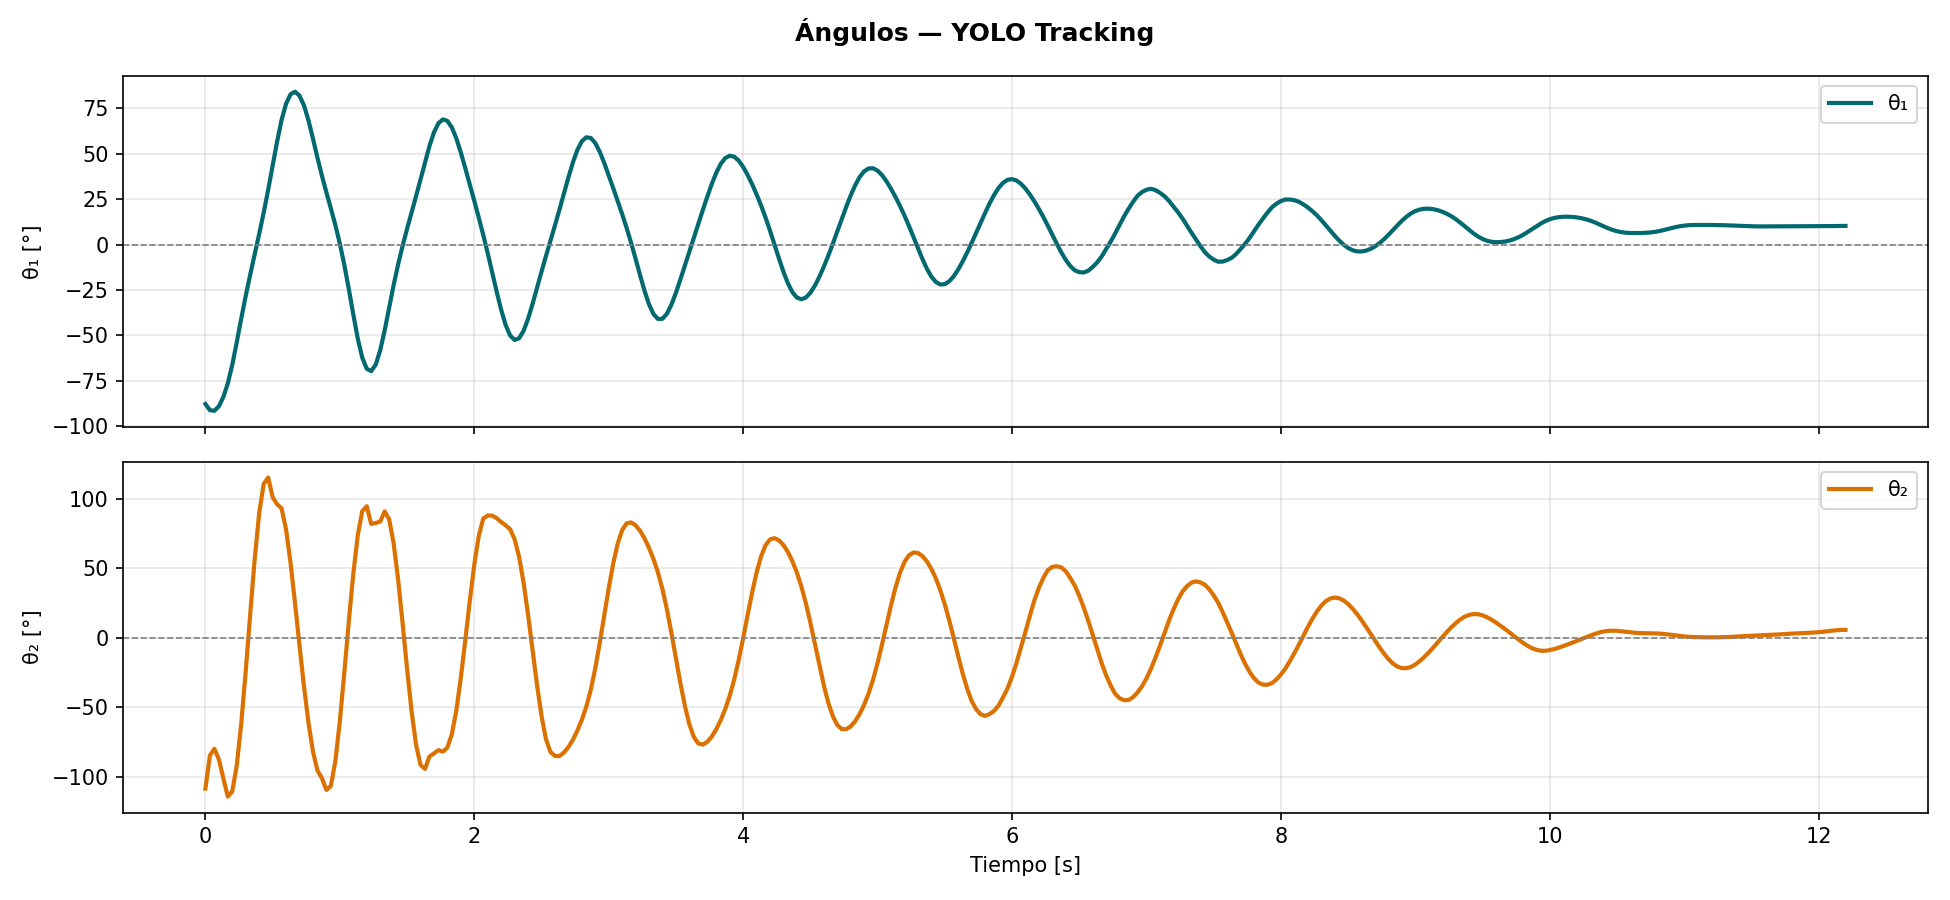
\includegraphics[width=0.4\textwidth]{plot_angles.png}
\caption{Ángulos \(\theta_1\) y \(\theta_2\) en el tiempo.}
\end{figure}

\section{Parámetros Identificados}
\begin{table}[H]
\centering
\begin{tabular}{lcc}
\toprule
Símbolo & Valor & Descripción \\
\midrule
\(L_1\) & 0.3743 m & Longitud barra 1 \\
\(L_2\) & 0.3714 m & Longitud barra 2 \\
\(m_1\) & 0.8285 kg & Masa eslabón 1 \\
\(m_2\) & 0.4203 kg & Masa eslabón 2 \\
\(b_1\) & 0.0329 N·m·s/rad & Amortiguamiento 1 \\
\(b_2\) & 0.5069 N·m·s/rad & Amortiguamiento 2 \\
\(g\) & 9.81 m/s² & Gravedad \\
\bottomrule
\end{tabular}
\caption{Parámetros identificados. Costo final: 4.447e-03}
\end{table}

\section{Modelo Matemático General}
Aplicando el método de Lagrange se obtienen las ecuaciones de movimiento:

\begin{align}
    & (m_1 + m_2)L_1 \ddot{\theta}_1 + m_2 L_2 \ddot{\theta}_2 \cos(\theta_1 - \theta_2) + m_2 L_2 \dot{\theta}_2^2 \sin(\theta_1 - \theta_2) \nonumber \\
    & \qquad + (m_1+m_2)g \sin\theta_1 + b_1 \dot{\theta}_1 = 0 \\[5pt]
    & m_2 L_2 \ddot{\theta}_2 + m_2 L_1 \ddot{\theta}_1 \cos(\theta_1 - \theta_2) - m_2 L_1 \dot{\theta}_1^2 \sin(\theta_1 - \theta_2) \nonumber \\
    & \qquad + m_2 g \sin\theta_2 + b_2 \dot{\theta}_2 = 0
\end{align}

\section{Modelo Numérico Identificado}
Sustituyendo los valores numéricos obtenidos:

\begin{align}
    & 0.467 \ddot{\theta}_1 
    + 0.156 \ddot{\theta}_2 \cos(\theta_1-\theta_2)
    + 0.156 \dot{\theta}_2^2 \sin(\theta_1-\theta_2) \nonumber \\
    & \qquad + 12.3 \sin\theta_1
    + 0.033 \dot{\theta}_1 = 0 \\[5pt]
    & 0.156 \ddot{\theta}_2
    + 0.157 \ddot{\theta}_1 \cos(\theta_1-\theta_2)
    - 0.157 \dot{\theta}_1^2 \sin(\theta_1-\theta_2) \nonumber \\
    & \qquad + 4.1 \sin\theta_2
    + 0.507 \dot{\theta}_2 = 0
\end{align}

\section{Análisis de Estabilidad (Linealización)}
Se linealizó el sistema alrededor de cuatro puntos de equilibrio. Los autovalores de la matriz \(A\) del sistema linealizado se muestran a continuación.

\begin{table}[H]
\centering
\begin{tabular}{lcc}
\toprule
Equilibrio & Autovalores (\(\lambda\)) & Tipo \\
\midrule
P1_colgante & $0.0000 + 7.9162i$, $0.0000 - 7.9162i$, $-0.0000 + 4.0806i$, $-0.0000 - 4.0806i$ & Silla \\
P2_semi_inv_b1 & $5.6703$, $-5.6703$, $-0.0000 + 5.6968i$, $-0.0000 - 5.6968i$ & Silla \\
P3_semi_inv_b2 & $5.6968$, $-0.0000 + 5.6703i$, $-0.0000 - 5.6703i$, $-5.6968$ & Silla \\
P4_invertido & $7.9162$, $4.0806$, $-7.9162$, $-4.0806$ & Silla \\

\bottomrule
\end{tabular}
\caption{Autovalores del sistema linealizado.}
\end{table}

\begin{figure}[H]
\centering
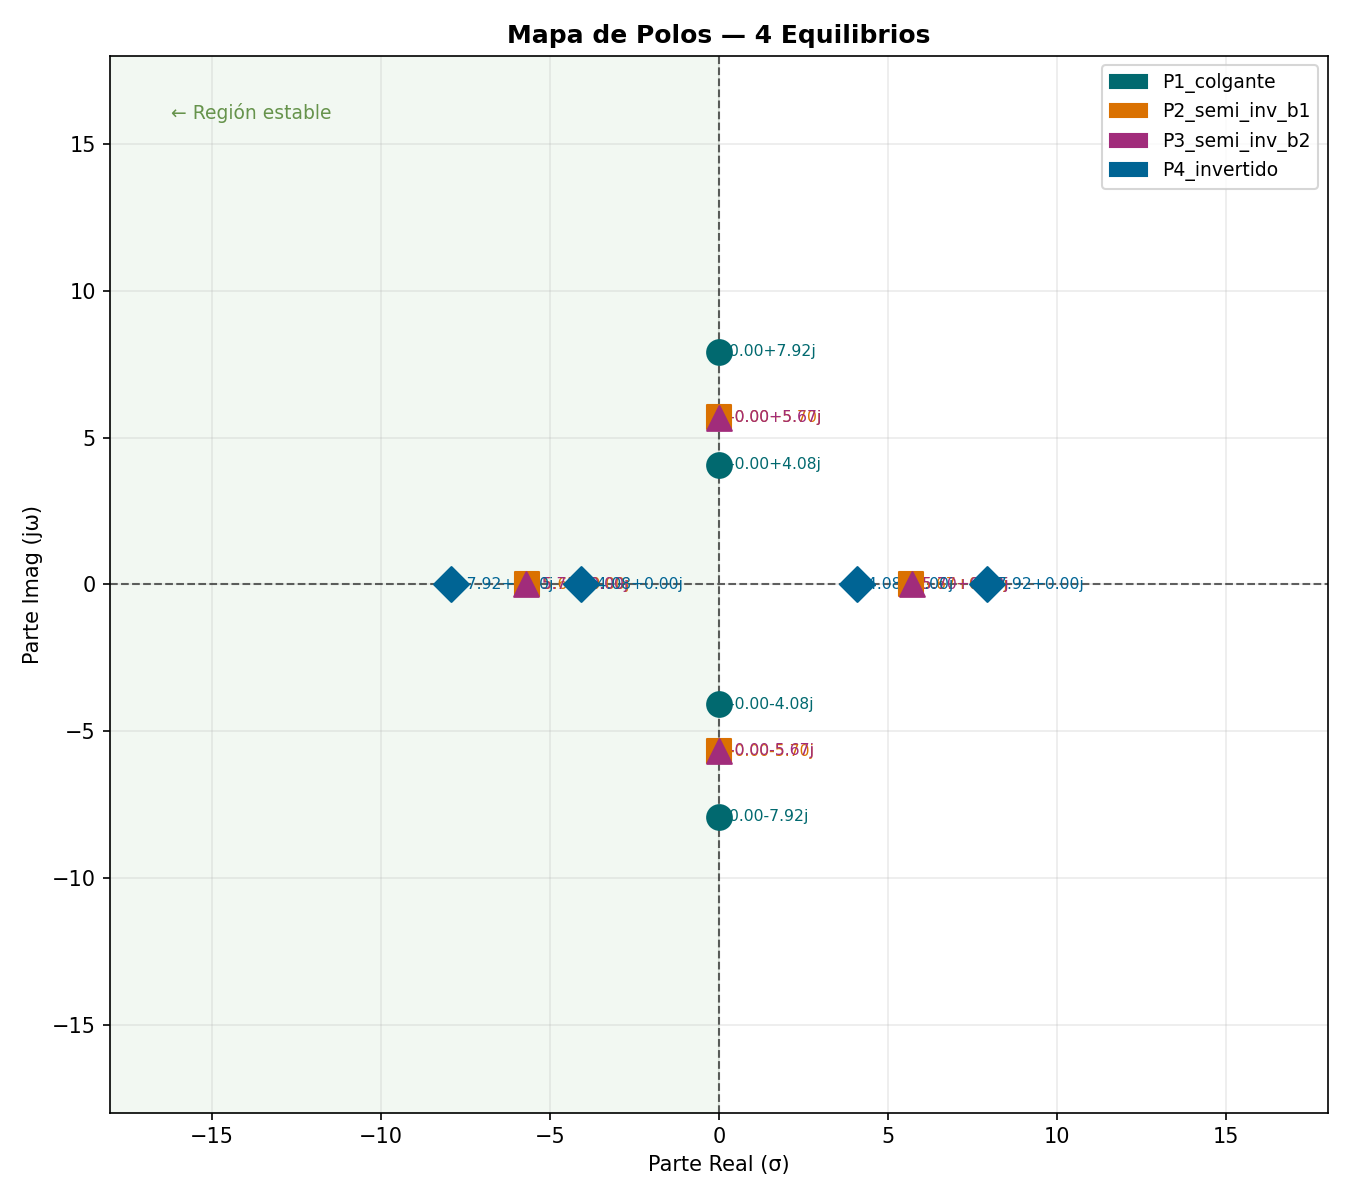
\includegraphics[width=0.7\textwidth]{plot_eigenvalues.png}
\caption{Ubicación de autovalores en el plano complejo.}
\end{figure}

\section{Representación en Espacio de Estados}
Definiendo el vector de estado \(\mathbf{x} = [\theta_1,\ \theta_2,\ \dot{\theta}_1,\ \dot{\theta}_2]^T\), el sistema se escribe como:

\[
\dot{\mathbf{x}} = \mathbf{f}(\mathbf{x}) = 
\begin{bmatrix}
\dot{\theta}_1 \\
\dot{\theta}_2 \\
\ddot{\theta}_1(\theta_1,\theta_2,\dot{\theta}_1,\dot{\theta}_2) \\
\ddot{\theta}_2(\theta_1,\theta_2,\dot{\theta}_1,\dot{\theta}_2)
\end{bmatrix}
\]

\section{Comportamiento Caótico}
Para oscilaciones de amplitud superior a \(20^\circ\) el péndulo doble presenta caos determinista: pequeñas variaciones en las condiciones iniciales producen trayectorias muy diferentes a largo plazo.

\section{Verificación Energética}
\begin{figure}[H]
\centering
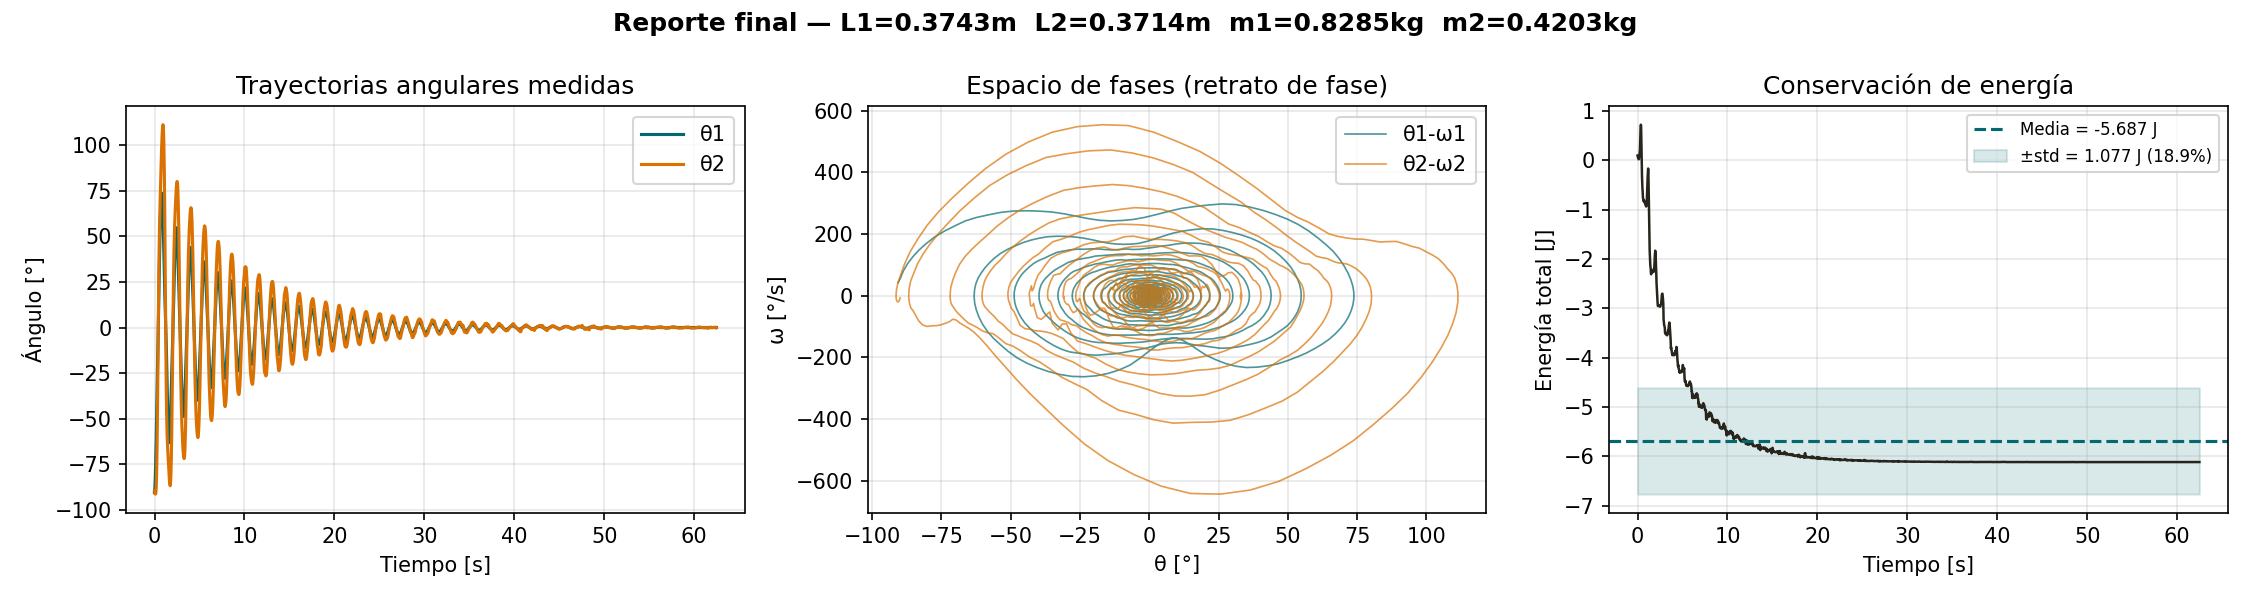
\includegraphics[width=0.7\textwidth]{plot_report.png}
\caption{Evolución de la energía total del sistema.}
\end{figure}

\end{document}
